\section{Implementazione}
\label{sec:implementazione}

\subsection*{Prima soluzione}

In questa relazione verranno discusse proprietà e risultati 
dell'algoritmo Hoshen-Kopelman \cite{Hoshen-Kopelman}.
Tuttavia, per dimostrarne la correttezza e provarne l'efficienza,
verranno effettuati dei confronti con una versione personalizzata,
che chiameremo algoritmo $A$,
la cui correttezza è ben nota data la sua semplicità.
Il Cod. \ref{alg:standard} mostra una prima soluzione 
al problema del partizionamento. È composto da 2 iterazioni principali: 
una ``esterna'' per tutti i siti occupati, una ``interna'' per i siti 
adiacenti. Quest'ultima si appoggia ad un vettore che 
funge da \textit{pila}, le cui dimensioni variano in maniera dinamica.
Lo scopo della pila è quello di aggiungere, ad ogni iterazione interna, 
i siti occupati adiacenti al nodo corrente, per essere poi processati
singolarmente.
Ragionando sul funzionamento del codice, ci si convince piuttosto 
facilmente della ridondanza causata dalla pila. In altri termini,
un sito occupato può essere processato più volte:
\begin{itemize}
    \item una e una sola volta nell'iterazione esterna;
    \item una volta per ogni vicino occupato;
    \item altre volte per eventuali ``catene di vicinanze''.
\end{itemize}

% Questo dettaglio fa sì che la complessità asintotica temporale \cite{sipser} 
% dell'algoritmo appartenga alla classe $\bigo{n^4}$ nel caso di un reticolo 
% bidimensionale $n \times n$. 

% \begin{lstlisting}[caption={Algoritmo standard di cluster-finding}, label={cod:cluster-finding}]
% function res = CercaCluster3(L, p)
% res.matrice=zeros(L+2);
% aux=rand(L)<p;
% res.matrice(2:end-1,2:end-1)=aux;
% res.percolazioneTB=0;
% res.percolazioneLR=0;
% res.cluSz=[];
% res.label=zeros(L+2);

% labelC=1;
% valid=find(res.matrice); % indici occupati

% for iter=1:length(valid)
%     ii=valid(iter);
%     if(res.label(ii)==0)
%         % nuovo cluster, esploro i vicini
%         pila=ii;
%         res.label(ii)=labelC;
%         j=1;
%         while(j<=length(pila))
%             elemento=pila(j);
%             % aggiungo i vicini alla pila
%             if(res.matrice(elemento-1) && res.label(elemento-1)==0)
%                 pila(end+1)=elemento-1;
%                 res.label(elemento-1)=labelC;
%             end
%             if(res.matrice(elemento+1) && res.label(elemento+1)==0)
%                 pila(end+1)=elemento+1;
%                 res.label(elemento+1)=labelC;
%             end
%             if (res.matrice(elemento-L-2) && res.label(elemento-L-2)==0)
%                 pila(end+1)=elemento-L-2;
%                 res.label(elemento-L-2)=labelC;
%             end
%             if (res.matrice(elemento+L+2) && res.label(elemento+L+2)==0)
%                 pila(end+1)=elemento+L+2;
%                 res.label(elemento+L+2)=labelC;
%             end
%             j=j+1;
%         end
%         res.cluSz(end+1)=length(pila); 
%         labelC=labelC+1;
%     end
% end


% res.label=res.label(2:end-1,2:end-1);
% res.matrice=res.matrice(2:end-1,2:end-1);
% left = clusters on the left edge
% right = clusters on the right edge
% if (~isempty(intersect(left,right)))
%     res.percolazioneLR=1;
% end

% auxT = unique(res.label(1:L:L*(L-1)+1));
% top = auxT(auxT>0);
% auxB = unique(res.label(L:L:L*L));
% bottom = auxB(auxB>0);
% if (~isempty(intersect(top, bottom)))
%     res.percolazioneTB = 1;
% end
% end
% \end{lstlisting}

\begin{algorithm}
    \caption{Pseudocodice dell'algoritmo $A$}
    \label{alg:standard}
    {\small
    \begin{algorithmic}[1]
    \State $largest\_label \gets 1$ 
    \State $label \gets \text{zeros}[n\_columns, n\_rows]$
    
    \For{$[x,y] \gets [0,0]$ \textbf{to} $n\_columns,n\_rows$}
        \If{$[x,y] = 1 \land label[x, y] = 0 $}
            \State $pila \gets [x, y]$ 
            \State $label[x, y] \gets largest\_label$
            \State $j \gets 1$
            
            \While{$j \leq \text{length}(pila)$}
                \State $elem \gets pila[j]$
                
                \State $x \gets elem[1], y \gets elem[2]$
                \State $left \gets [x - 1, y]$
                \State $right \gets [x + 1, y]$
                \State $down \gets [x, y+1]$
                \State $top \gets [x, y-1]$
                
                \If{$left = 1 \land label[left] = 0$}
                    \State $\text{append } left \text{ to } pila$
                    \State $label[left] \gets largest\_label$
                \EndIf
                
                \If{$right = 1 \land label[right] = 0$}
                    \State $\text{append } right \text{ to } pila$
                    \State $label[right] \gets largest\_label$
                \EndIf
                
                \If{$up = 1 \land label[up] = 0$}
                    \State $\text{append } up \text{ to } pila$
                    \State $label[up] \gets largest\_label$
                \EndIf
                
                \If{$down = 1 \land label[down] = 0$}
                    \State $\text{append } down \text{ to } pila$
                    \State $label[down] \gets largest\_label$
                \EndIf
                
                \State $j \gets j + 1$
            \EndWhile
            
            \State $largest\_label \gets largest\_label + 1$
        \EndIf
    \EndFor
    \end{algorithmic}
    }
\end{algorithm}

\subsection*{Paradigma Union-Find}

Come appena accennato, in questa relazione viene presentato l'algoritmo 
Hoshen-Kopelman, che fa parte della famiglia di algoritmi \textit{union-find},
utilizzati nel calcolo di componenti connesse e, in questo caso, per il processo 
di cluster-finding. Questo paradigma prevede l'utilizzo di due procedure principali, che 
ne compongono il nome:
\begin{itemize}
    \item \textit{Union}: effettua una fusione tra due insiemi disgiunti quando ci 
    si accorge che appartengono in realtà alla stessa classe di equivalenza;
    \item \textit{Find}: determina a quale insieme appartiene l'elemento in elaborazione.
\end{itemize}

\begin{algorithm}
    \caption{Pseudocodice dell'algoritmo Hoshen-Kopelman}
    \label{alg:HK}
    {\small
    \begin{algorithmic}[1]
    \State $largest\_label \gets 0$
    \State $label \gets \text{zeros}[n\_columns, n\_rows]$
    \State $Lofl \gets [0:n\_columns]$
    \\
    \For{$[x,y] \gets [0,0]$ \textbf{to} $[n\_columns,n\_rows$}
        \If{$[x, y] = 1$}
            \State $left \gets label[x-1, y]$
            \State $above \gets label[x, y-1]$
            \If{$(left = 0) \land (above = 0)$}
                \State $largest\_label \gets largest\_label + 1$
                \State $tmp \gets largest\_label$
            \ElsIf{$(left = 1) \land (above = 0)$}
                \State $tmp \gets left$
            \ElsIf{$(left = 0) \land (above = 1)$}
                \State $tmp \gets above$
            \Else
                \State $tmp \gets \text{min}\{left,above\}$
                \State $bad\_label \gets \text{max}\{left,above\}$
                \State $\Call{Union}{bad\_label, tmp}$
            \EndIf
            \State $label[x,y] \gets tmp$
        \EndIf
    \EndFor
    
    \vspace{5pt}
    \Procedure{Union}{$x, y$}
        \State $Lofl[\Call{Find}{x}] \gets \Call{Find}{y}$
    \EndProcedure

    \vspace{5pt}
    \Function{Find}{$x$}
        \While{$Lofl[x] \neq x$}
            \State $x \gets Lofl[x]$
        \EndWhile
        \State \Return $x$
    \EndFunction
    
    \end{algorithmic}
    }
\end{algorithm}

Nel Cod. \ref{alg:HK} vengono mostrati i passaggi per l'implementazione 
del paradigma nel contesto della percolazione \cite{pseudoHK}.
Rispetto all'algoritmo iniziale, rimane un'iterazione sui siti per verificarne
l'occupazione, ma appare diversa la logica applicata. In particolare, scompare
l'utilizzo della pila con la conseguente ridondanza e, per 
ogni sito occupato, vengono considerati solo due primi vicini: sopra (\textit{$above$}) 
e a sinistra ($left$). Se nessuno dei due vicini è occupato, al sito 
viene assegnata una nuova etichetta ($label$), aggiornata tramite un contatore;
se soltato uno dei due vicini è occupato, il sito eredita la sua etichetta;
se entrambi i vicini sono occupati e hanno la stessa etichetta, il comportamento
è analogo al caso di un vicino occupato; se invece i vicini hanno etichette diverse, 
il sito eredita quella minore, prestando attenzione al fatto che in realtà 
le due facciano riferimento allo stesso cluster.
Infatti, in questo procedimento si possono avere siti di uno 
stesso cluster con etichette diverse (provare per credere!).
Quest'ultimo punto è cruciale: è necessario tenere conto di questa informazione
senza impattare negativamente sul costo computazionale dell'algoritmo; una rinomina
totale delle etichette sarebbe infatti troppo costosa e si perderebbe parte del vantaggio
ottenuto rispetto all'algoritmo $A$.
Per coprire questo aspetto, per ogni cluster si sceglie una etichetta 
``di rappresentanza'', che chiameremo \textit{good label}. Ogni altra etichetta viene 
considerata una \textit{bad label} e deve essere in qualche modo collegata alla rispettiva
\textit{good label}. Il metodo di collegamento scelto consiste nell'utilizzo di un array 
$Lofl$ (Label of label), che viene aggiornato durante l'esecuzione. 
A questo proposito, entrano in gioco le nuove procedure:
\begin{itemize}
    \item \textit{Union}: ha il compito di collegare una \textit{bad label} ad una 
    potenziale\footnotemark{} \textit{good label} e viene descritta facilmente in termini di \textit{Find};
    \item \textit{Find}: viene implementata come iterazione di punto fisso 
        della funzione rappresentata dall'array $Lofl$. In 
        altri termini, si cerca in modo iterativo la condizione di arresto $Lofl[x]=x$.
\end{itemize}
\footnotetext{Il termine ``potenziale'' fa riferimento al fatto che non sia possibile 
sapere se l'etichetta minore sia effettivamente una \textit{good label}, 
perché potrebbe a sua volta far parte di un altro collegamento. Tuttavia, si può dire che tramite una catena di 
collegamenti è possibile risalire alla \textit{good label}.}

\subsection*{Stime della soglia ed errori associati}
Per stabilire in maniera formale se esista o meno un cluster percolante (ricordiamo: un cluster 
percolante attraversa l'intero reticolo), va fatto un confronto tra le etichette presenti sui bordi
del reticolo: se esiste almeno un'etichetta presente su due bordi opposti, significa che il cluster 
identificato da esso attraversa il reticolo in quella direzione. 
Nell'algoritmo $A$ è sufficiente confrontare le etichette, mentre per Hoshen-Kopelman occorre 
confrontare le \textit{good label} dei siti presenti sui bordi.
Il processo consiste nel verificare che vi sia una intersezione non nulla tra le etichette 
presenti sul bordo sinistro e quelle sul bordo destro (left-right) oppure, in maniera analoga,
tra il bordo più alto e quello più basso (top-bottom).
Un paragone tra le rilevazioni dei due algoritmi mostrerà come i risultati ottenuti nei due casi 
siano perfettamente coincidenti.
% \begin{figure}[ht]
%     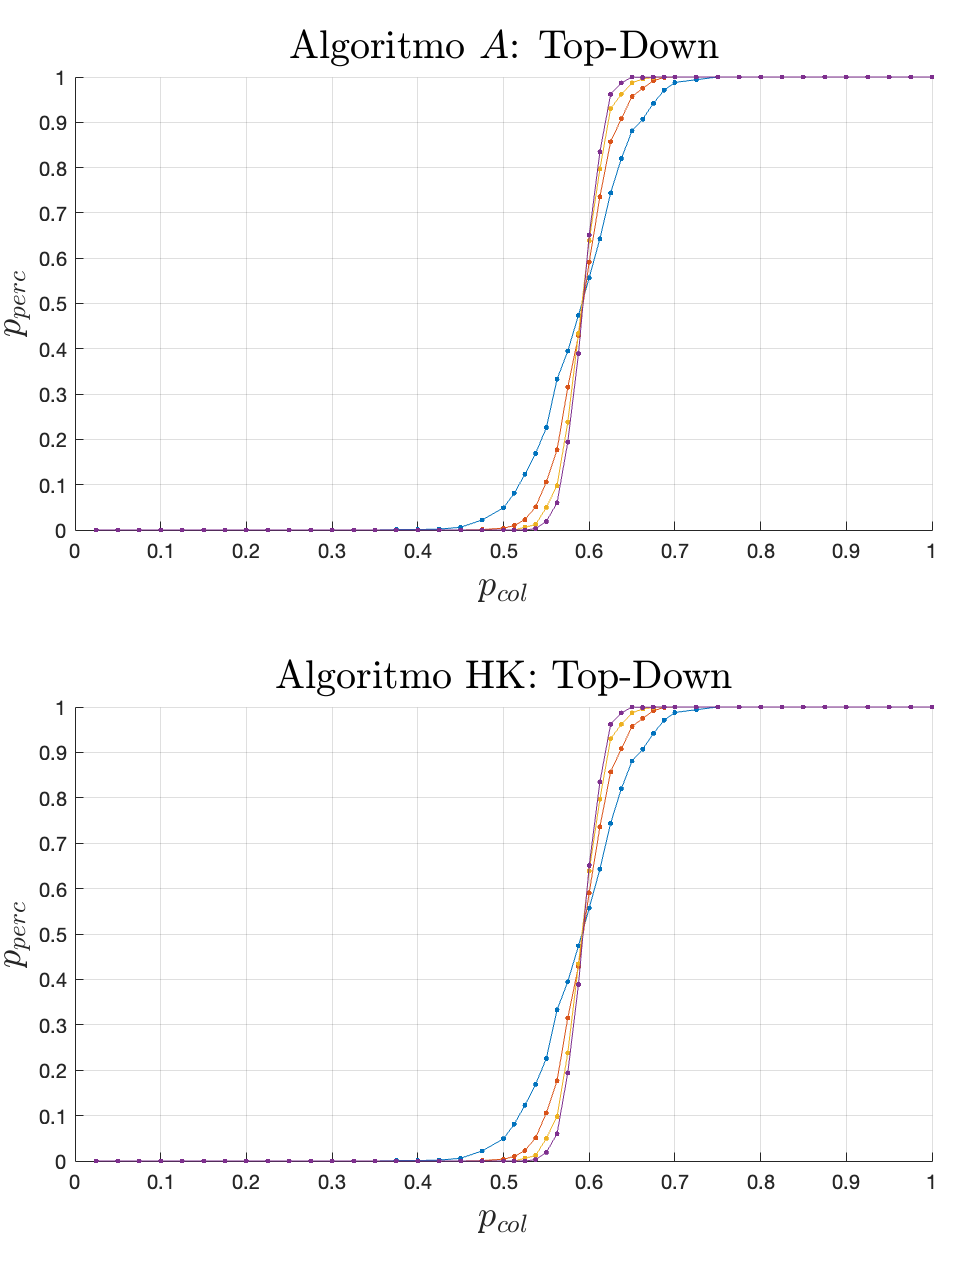
\includegraphics[width=0.9\columnwidth]{compare_threshold_1.png}
%     \caption{Confronto tra soglie di percolazione top-down calcolate dai due algoritmi.}
%     \label{fig:compare_threshold}
% \end{figure}
Per generare valori significativi ed effettuare confronti tra gli algoritmi, è stato necessario 
definire valori dei parametri richiesti nella simulazione e iterare su di essi.
Si è definito un array $L = [20,60,40,80]$ per le dimensioni.
Si è costruito un array $p$ per le probabilità di occupazione, tramite punti non equidistanti:
\begin{enumerate}
    \item $p_a = [0.025:0.025:0.5]$;
    \item $p_b = [0.5125:0.0125:0.7]$;
    \item $p_c = [0.725:0.025:1]$;
    \item $p = [p_a,p_b,p_c]$.
\end{enumerate}
La sintassi utilizzata richiama volontariamente quella del linguaggio Matlab: 
la scritta $[inf : inc : sup]$ indica una serie di valori che parte da $inf$ e arriva
a $sup$, tramite un incremento costante $inc$.
Si è scelto infine un numero arbitrario $N$ di iterazioni per determinare, fissando 
i parametri precedenti, la frequenza
di percolazione, calcolata banalmente dividendo $n_{perc}$ (numero di esperimenti in 
cui avviene percolazione) per $N$, in questo caso uguale a $1000$. 
\begin{equation}
    \forall i \in [1..N] : 
    \begin{cases}
        t(i) = 1 ,& \text{se avviene percolazione} \\
        t(i) = 0 ,& \text{altrimenti}.
    \end{cases}
\end{equation}
Per ogni test $i \in [1..N]$ vi sono quindi 2 casi: avviene o non avviene percolazione.
I risultati dei test sono memorizzati all'interno di un array $t$ tramite valori di verità. 
Si denota con $t(i) \in \{0,1\}$ il risultato dell'$i$-esimo test a parametri fissati.
Grazie alla notazione introdotta, si nota facilmente che:
\begin{equation}
    \sum_{i=1}^{N} t(i) = n_{perc}
\end{equation}
Seguendo questi passaggi, si può valutare $t(i)$ come se fosse una misurazione di una 
variabile aleatoria $T$.
Si può pensare che $T$ segua una legge di distribuzione binomiale della forma
\begin{equation*}
    T \sim \mathcal{B}_{n,p}(k)
\end{equation*} 
Ma che tipo di binomiale? Si potrebbe attribuire $n=N$ e chiaramente siamo interessati a $k=n_{perc}$.
Tuttavia, non si conoscono i valori esatti del parametro $p_{perc}$ sulla probabilità di percolazione e 
occorre quindi procedere per \textit{stime}.
Il fatto che la frequenza di percolazione sia significativa rispetto alla probabilità 
della stessa è garantito, per input sufficientemente grandi, dalla \textbf{\textit{Legge dei Grandi Numeri}}
espressa in forma di Chebyshev \cite{big-numbers, chebyshev}.
L'affidabilità delle misurazioni effettuate è invece discussa per mezzo del 
\textbf{\textit{Teorema del Limite Centrale (TLC)}} \cite{tlc}.
Questi strumenti matematici permettono di affermare proprietà statistiche sulle 
stime del parametro $p_{perc}$ e sull'errore associato. Formalmente, si calcola 
la media aritmetica sugli esperimenti come 
\begin{equation}
    f_{perc} = \frac{n_{perc}}{N} = \frac{1}{N} \sum_{i=1}^{N} t(i)
\end{equation}
Sappiamo da \ref{eq:lgn} che, per $N$ sufficientemente grande, $f_p$ converge 
in probabilità al valore atteso di $T$. Inoltre, la varianza associata è
\begin{equation}
    D_{f_{perc}} = \frac{1}{N^2} \sum_{i=1}^{N} {D}_T = \frac{{D}_T}{N}
\end{equation}
dove $D_T$ è la varianza della variabile aleatoria $T$ e può essere stimata 
in Matlab seguendo le misurazioni del campione:
\begin{equation}
    \tilde{D}_T = D_t = \frac{1}{N-1} \sum_{i}^{N} \left(t(i) - f_{perc}\right)^2
\end{equation}
Ci si avvale a questo punto anche dell'equazione \ref{eq:tlc} e ne consegue che 
\begin{equation}
    f_{perc} \sim \mathcal{N}(\sigma^2, \mu) = \frac{1}{\sqrt{2\pi\sigma^2}} e^{-\frac{(x - \mu)^2}{2\sigma^2}}
\end{equation}
o, in altri termini, la frequenza di percolazione rilevata nella simulazione segue una legge 
di distribuzione gaussiana. 
Si può dire di più: i parametri della funzione sono proprio le stime effettuate sul campione.
Questi passaggi risultano molto importanti perché permettono di ricondurre
esperimenti ``arbitrari'' a casistiche ben note. Sostanzialmente, conoscendo la natura
della distribuzione gaussiana, ci è concesso affermare che valori lontani 
dalla media $\mu=f_{perc}$ per più di $3\sigma$, dove $\sigma=\sqrt{\tilde{D}_T}$, possano essere esclusi
dai candidati per il valore esatto $p_{perc}$. Partendo dai campioni restituiti dalla simulazione,
si è quindi arrivati a costruire un \textit{intervallo di confidenza} all'interno del quale il valore ricercato ha probabilità 
$1-\alpha$ di apparire, dove $\alpha$ rappresenta l'area sottesa dalla funzione di densità $f_{perc}$ negli intervalli $(-\infty, \mu - 3\sigma)$
e $(\mu + 3\sigma, +\infty)$.
In Fig. \ref{fig:f_perc_pdf} è mostrato un esempio grafico per capire meglio il concetto.
\begin{figure}[ht]
    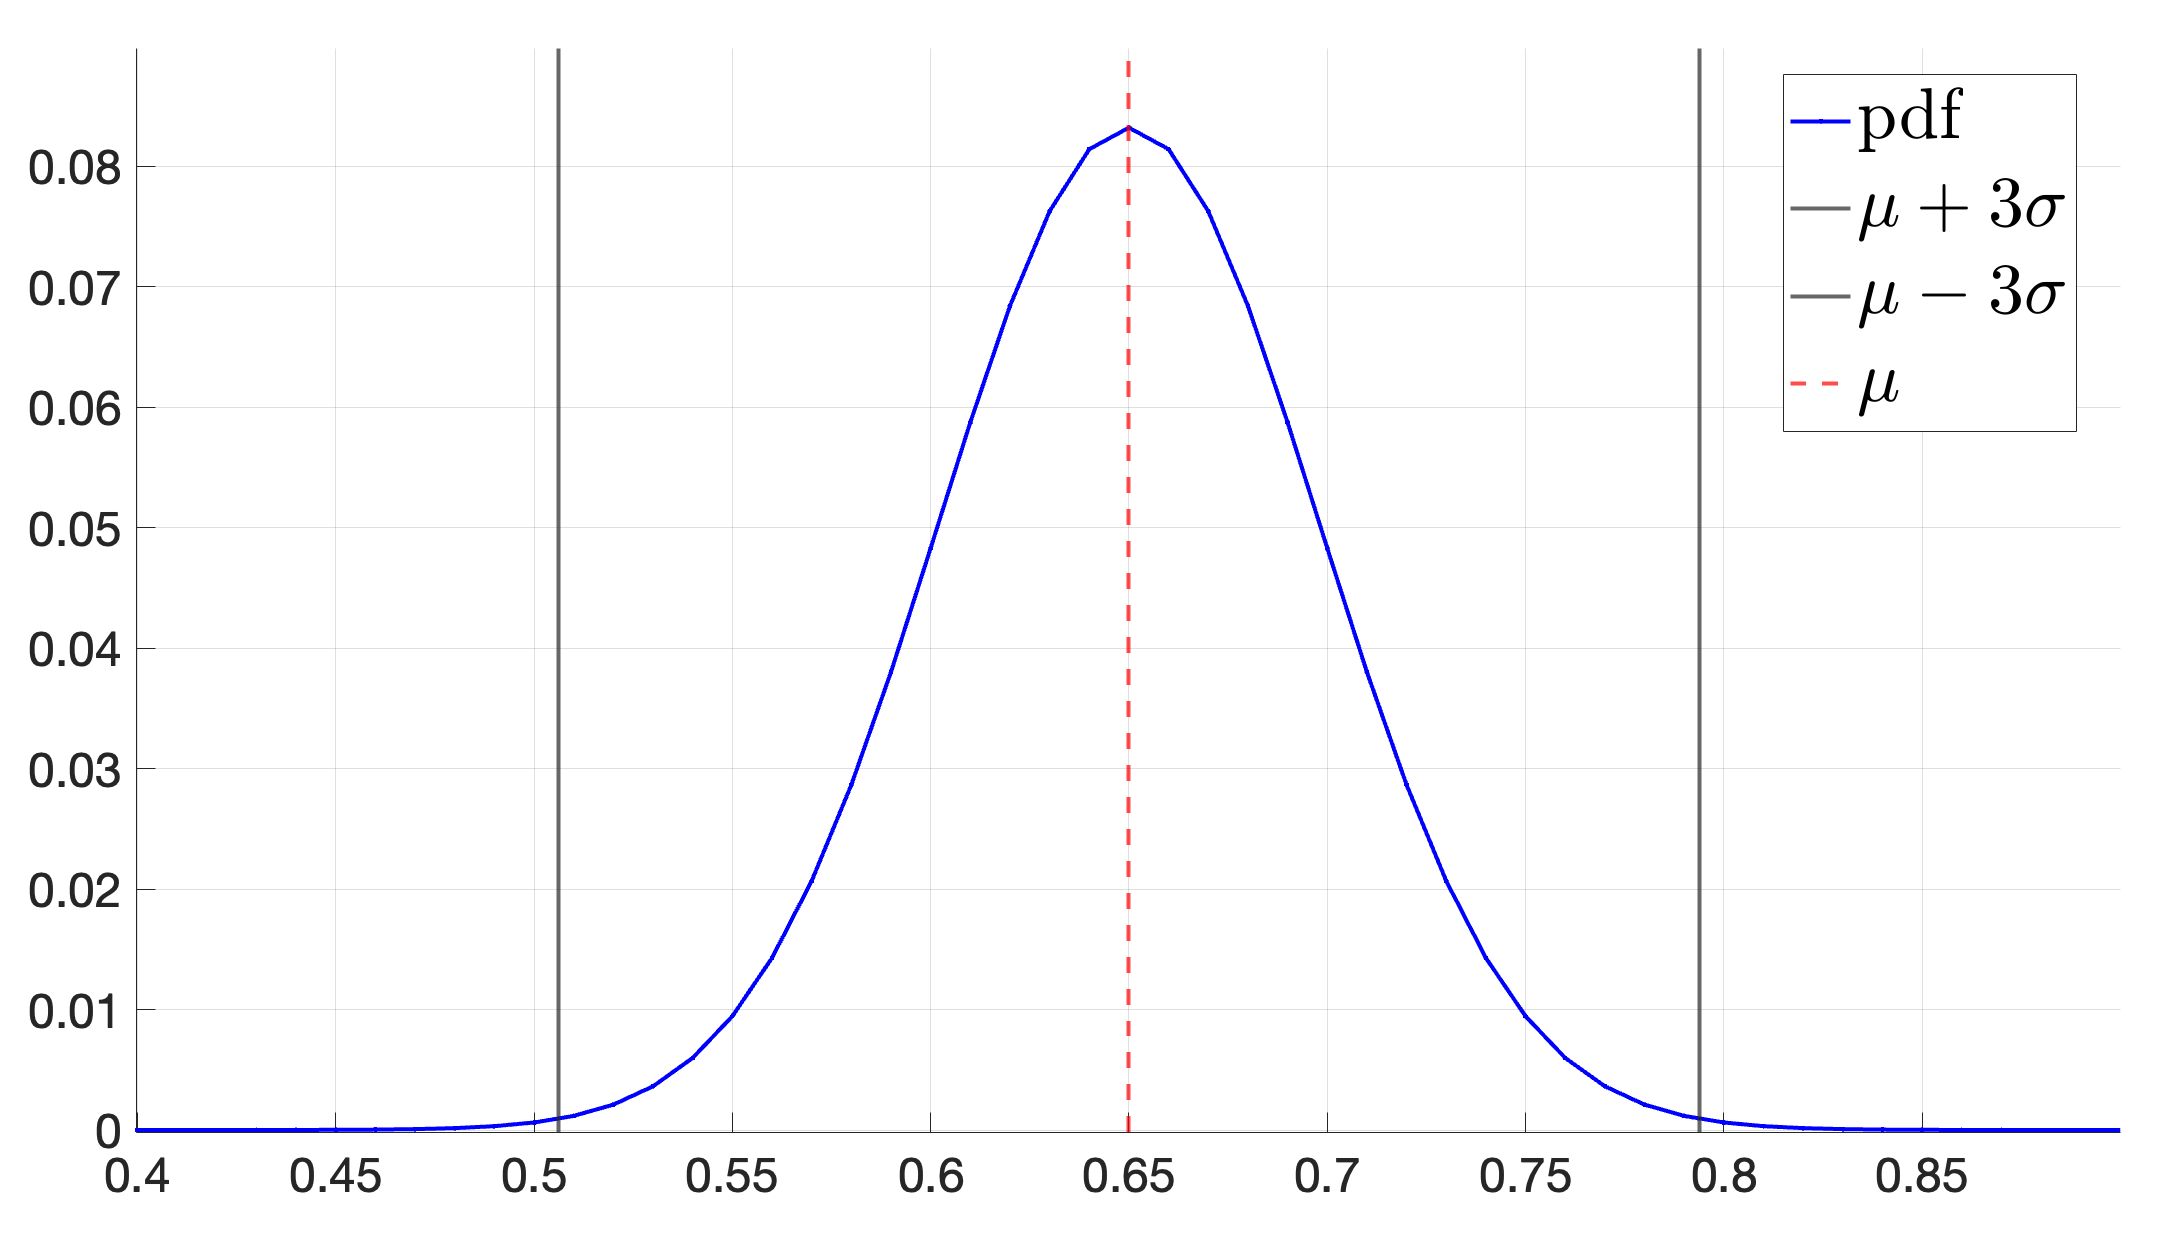
\includegraphics[width=\columnwidth]{f_perc_pdf.png}
    \caption{Funzione di densità probabilistica normale per $f_{perc}$.}
    \label{fig:f_perc_pdf}
\end{figure}

\subsection*{Altre osservabili}
Si può svolgere il procedimento di stima dei parametri di una distribuzione non conosciuta anche per 
altre quantità, dette ``osservabili''. Ognuna di queste, nel nostro caso, è riconducibile ad una 
funzione gaussiana per lo stesso motivo descritto nel paragrafo precedente legato a TLC.
Anche la correttezza della stima si discute nel senso di convergenza in probabilità, come già mostrato.
Di seguito è esposta una panoramica delle osservabili studiate, oltre alla frequenza di percolazione.
\subsubsection*{$P_1$}
Rappresenta la probabilità che il cluster più grande trovato (dimensione $s_{max}$) sia grande 
quanto l'intero reticolo. È lecito pensare (e si avrà una conferma) che questa quantità sia 
trascurabile per valori piccoli della probabilità di occupazione $p$, e avrà andamento crescente
fino a $p=1$, dove sicuramente vi sarà un unico cluster di dimensione $s_{max}$.
\begin{equation}
    P_1=\frac{s_{max}}{|L|}
\end{equation}
\subsubsection*{$P_2$}
Rappresenta la probabilità che il cluster più grande trovato sia grande 
quanto il numero medio di siti occupati. Occorre fare una precisazione:
I valori di questa quantità potrebbero essere superiori ad 1, poiché il 
denominatore è soltato una stima tramite valore medio (numero di siti 
moltiplicati per la probabilità di occupazione).
Anche in questo caso, comunque, ci si aspetta un andamento simile al precedente.
\begin{equation}
    P_2=\frac{s_{max}}{p |L|}
\end{equation}
\subsubsection*{$P_3$}
Rappresenta la probabilità che il cluster più grande trovato sia grande 
quanto il numero esatto di siti occupati. In questo caso, rispetto a $P_2$,
al denominatore è presente un valore calcolato analiticamente. Questa differenza
elimina la presenza di valori anomali maggiori di 1, ma la quantità calcolata,
soprattutto per un numero elevato di tentativi, rimane molto simile.
\begin{equation}
    P_3 = \frac{s_{max}}{\sum_s s \cdot n_s}
\end{equation}
\subsubsection*{$RACS$}
Rappresenta la probabilità che un sito appartenga ad un cluster che non sia quello 
di dimensone massima. In questo caso, ci si aspetta un andamento ``opposto'' rispetto 
alle altre quantità: per probabilità alte di occupazione è più probabile avere un cluster
che sia molto più grande degli altri, di conseguenza la probabilità che un sito vi appartenga 
è più bassa.
\begin{equation}
    RACS = \frac{\sum_{s\neq s_{max}} s \cdot n_s}{\sum_t t \cdot n_t}
\end{equation}
